\iffalse
\let\negmedspace\undefined
\let\negthickspace\undefined
\documentclass[journal,12pt,twocolumn]{IEEEtran}
\usepackage{cite}
\usepackage{amsmath,amssymb,amsfonts,amsthm}
\usepackage{algorithmic}
\usepackage{graphicx}
\usepackage{textcomp}
\usepackage{xcolor}
\usepackage{txfonts}
\usepackage{listings}
\usepackage{enumitem}
\usepackage{mathtools}
\usepackage{gensymb}
\usepackage{comment}
\usepackage[breaklinks=true]{hyperref}
\usepackage{tkz-euclide} 
\usepackage{listings}
\usepackage{gvv}                                        
\def\inputGnumericTable{}                                 
\usepackage[latin1]{inputenc}                                
\usepackage{color}                                            
\usepackage{array}                                            
\usepackage{longtable}                                       
\usepackage{calc}                                             
\usepackage{multirow}                                         
\usepackage{hhline}                                           
\usepackage{ifthen}                                           
\usepackage{lscape}

\newtheorem{theorem}{Theorem}[section]
\newtheorem{problem}{Problem}
\newtheorem{proposition}{Proposition}[section]
\newtheorem{lemma}{Lemma}[section]
\newtheorem{corollary}[theorem]{Corollary}
\newtheorem{example}{Example}[section]
\newtheorem{definition}[problem]{Definition}
\newcommand{\BEQA}{\begin{eqnarray}}
\newcommand{\EEQA}{\end{eqnarray}}
\newcommand{\define}{\stackrel{\triangle}{=}}
\theoremstyle{remark}
\newtheorem{rem}{Remark}

\usepackage{graphicx}
\graphicspath{ {./Downloads/} }
\begin{document}

\bibliographystyle{IEEEtran}
\vspace{3cm}

\title{ASSIGNMENT 1}
\author{EE22BTECH11060 - TEJAVATH KUSHAL$^{*}$% <-this % stops a space
}
\maketitle
\newpage
\bigskip

\renewcommand{\thefigure}{\theenumi}
\renewcommand{\thetable}{\theenumi}


\maketitle
QUESTION 17:\\
A man starts repaying a loan as first instalment of Rs.$100$. If he increases the
instalment by Rs $5$ every month, what amount he will pay in the $30^{th}$ instalment?\\

SOLUTION:\\
\fi
\begin{table}[ht]
\setlength{\arrayrulewidth}{0.3mm}
\setlength{\tabcolsep}{15pt}
\renewcommand{\arraystretch}{1.5}



\begin{tabular}{ |p{1cm}|p{2cm}|p{2cm}| }
\hline
Parameter & Value & Description\\
\hline
$x(n)$ & $(x(0)+nd)u(n)$ & general term \\ \hline
$x(0)$ & $100$ & first term\\ \hline
$d$ & $5$ & Common difference\\ \hline
$x\brak{29}$ & $\brak{x\brak{0} + 29d}u\brak{n}$ & $30^{th}$term\\ \hline 

%$x(l)$ & Last($l^{th}$) term of series & 350\\
%$x(0)$ & Starting ($0^{th}$) term of series & 17 %\\
%\hline
%d & Common difference of AP & 9\\
%\hline
\end{tabular}
\caption{Parameters}



\end{table}

\begin{align}
x(n)&= 100 + 5n \\
x(29)&= x(0)+29d \\
x(29)&= 100+ 145 \\
x(29)&= 245
\end{align}
Z transform of $x(n)= 100 + 5n$,
\begin{align}
X \brak{z} & = \sum_{n=-\infty}^{\infty} x \brak{n}   z^{-n} \\
& = \sum_{n=-\infty}^{\infty}  \brak{100+5n} u \brak{n}   z^{-n} \\
\notag & = \sum_{n=-\infty}^{\infty} \brak{100} u \brak{n}   z^{-n} \\  &~~~~~~~+\sum_{n=-\infty}^{\infty} \brak{5n} u \brak{n}  z^{-n} \\
\implies X \brak{z} & = \frac{100}{1-z^{-1}} + \frac{5z^{-2}}{\brak{1-z^{-1}}^2} \\
ROC &: \abs{z} > 1 \notag
\end{align}


\pagebreak

\begin{figure}[h]
    %\caption{Stem Plot of $x\brak{n}$ v/s n}
    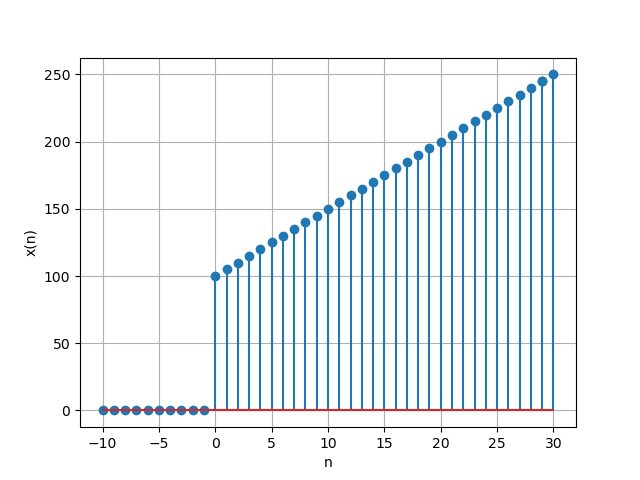
\includegraphics[width=0.5\textwidth]{ncert-maths/11/9/2/17/figs/x(n)_vs_n.png}
    \caption{Stem Plot of $x\brak{n}$ v/s n}
\end{figure}
%\end{document}
